\subsection{Verificação técnica do assistente}
\label{subsec:verificacao-interface}

A verificação técnica examinou a primeira etapa do assistente de personalização com três perguntas: se a etapa pode ser percorrida por teclado, se o leiaute se adapta a larguras de computador e de celular sem rolagem horizontal e quais problemas de acessibilidade uma ferramenta automática encontra nessa tela. Foi uma inspeção automatizada, sem participantes. Nenhuma pessoa usou a interface durante a verificação, de modo que não houve instruções a usuários, intervenções nem observação de uso; os dados vêm apenas das medições feitas pelo \textit{script} descrito a seguir.

\subsubsection{Ferramentas e ambiente}

A verificação foi feita por um \textit{script} em Node.js, \texttt{verificar-interface.cjs}, que conduz o navegador pelo Playwright e executa a análise de acessibilidade com o axe-core por meio do pacote \texttt{@axe-core/playwright}. As versões registradas foram Node.js 25.2.1, Playwright 1.63.0, axe-core 4.13.0 e Chromium 153.0.8010.12, este executado sem interface gráfica (\textit{headless}). A aplicação rodou localmente, no servidor de desenvolvimento do Next.js, e a rota examinada foi \texttt{/language-creator}, aberta sem autenticação e sem consulta a contas.

O \textit{script} combina dois temas, claro e escuro, com duas janelas, de 1440 por 1000 e de 390 por 844 pixels CSS, o que dá quatro cenários. Em todos eles, o navegador recebe a preferência por movimento reduzido, e o portal de ferramentas de desenvolvimento do Next.js é ocultado e excluído da análise, porque não faz parte da aplicação. A verificação foi executada pela primeira vez em 12 de setembro de 2026 e repetida em 16 de setembro, sobre a versão \texttt{b4372bf}, com o mesmo procedimento e as mesmas versões das ferramentas. Os resultados apresentados nesta seção são os da execução de 16 de setembro.

\subsubsection{Roteiro e critérios}

Em cada cenário, o \textit{script} segue o mesmo roteiro:

\begin{enumerate}
    \item abre a rota, confere que ela responde com o código HTTP 200 e aguarda a lista de etapas, a aplicação do tema e o carregamento das fontes;
    \item captura a tela e mede a largura da janela, a largura de rolagem do documento, a direção da lista de etapas e o posicionamento dos rótulos das etapas;
    \item pressiona Tab até o foco chegar ao botão da primeira etapa, com limite de 80 acionamentos;
    \item pressiona Tab e Enter e confere que o título da etapa ativa passou a ser ``Entrada/Saída'';
    \item pressiona Shift+Tab e Enter e confere o retorno à etapa ``Identidade'';
    \item executa o axe com as regras dos níveis A e AA das WCAG~2.0, 2.1 e 2.2 disponíveis na ferramenta.
\end{enumerate}

Os critérios de aprovação estão no próprio \textit{script}. A rota deve responder com o código 200, a primeira etapa deve ser alcançada por Tab dentro do limite e as duas transições por Enter devem mudar o título da etapa ativa; se uma dessas condições falha, a execução é interrompida. Para o leiaute, a ausência de rolagem horizontal é verificada pela igualdade entre a largura de rolagem do documento e a largura da janela. As ocorrências do axe não têm critério de aprovação: o relatório guarda, para cada cenário, as violações por regra, os elementos afetados e os itens que a ferramenta classificou como inconclusivos.

\subsubsection{Resultados}

A verificação abrangeu a etapa inicial do assistente e a navegação para a etapa de entrada e saída; não incluiu contas, turmas, submissões nem uso de leitor de tela. Nos quatro cenários, cinco acionamentos de Tab alcançaram o botão da primeira etapa, e Tab seguido de Enter ativou a segunda etapa. A lista de etapas apresentou direção vertical em 1440 pixels e horizontal em 390 pixels. A largura de rolagem do documento coincidiu com a largura da janela nos dois tamanhos. Esses resultados caracterizam o estado testado, não todos os componentes e estados da plataforma.

A Figura~\ref{fig:responsividade-wizard} mostra a captura no tema escuro com a janela de 1440 pixels, em que as etapas ficam na lateral e o conteúdo se organiza em colunas.

\begin{figure}[H]
\centering
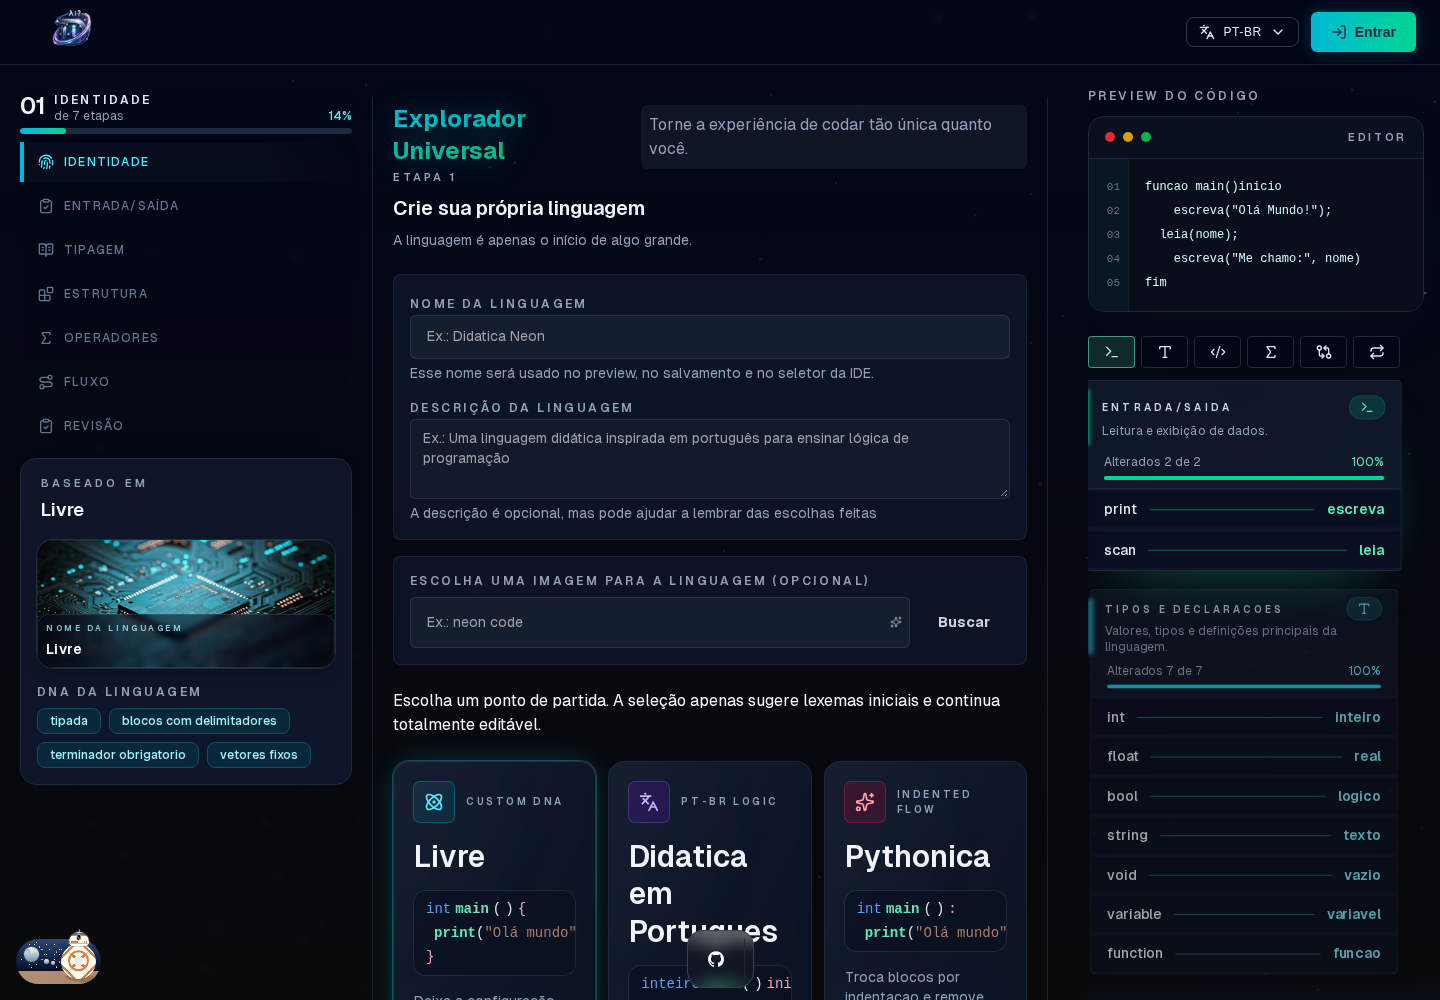
\includegraphics[width=\textwidth,height=0.40\textheight,keepaspectratio]{wizard-desktop-2026-09-16.png}
\caption{Assistente na versão verificada em setembro de 2026, em janela de 1440 por 1000 pixels CSS: etapas na lateral e conteúdo em colunas.}
\label{fig:responsividade-wizard}
\legend{Fonte: captura local da aplicação, sem autenticação.}
\end{figure}

Com a janela de 390 pixels, as etapas passam para uma linha no alto da tela e os cartões ficam empilhados, como mostra a Figura~\ref{fig:responsividade-wizard-celular}.

\begin{figure}[H]
\centering
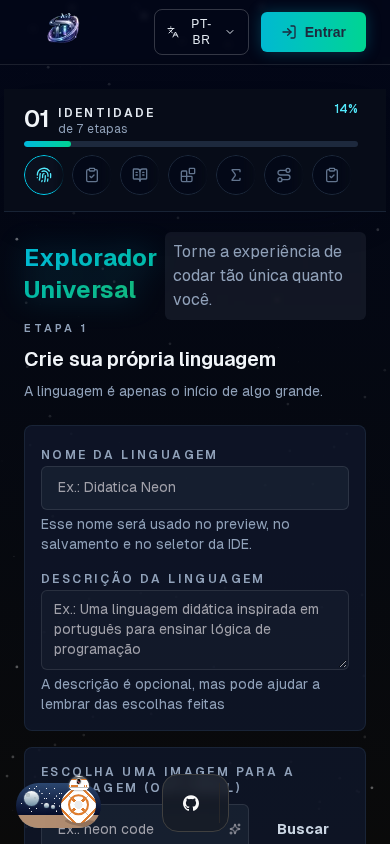
\includegraphics[height=0.32\textheight,keepaspectratio]{wizard-mobile-2026-09-16.png}
\caption{Assistente na versão verificada em setembro de 2026, em janela de 390 por 844 pixels CSS: etapas em linha e cartões empilhados.}
\label{fig:responsividade-wizard-celular}
\legend{Fonte: captura local da aplicação, sem autenticação.}
\end{figure}

A Tabela~\ref{tab:verificacao-axe} resume as ocorrências reportadas pelo axe por regra e cenário. Uma ocorrência corresponde a um elemento identificado pela ferramenta; as contagens de cenários distintos não devem ser somadas como problemas únicos. O relatório também contém itens inconclusivos, sobretudo de contraste, que requerem inspeção manual.

\begin{table}[htbp]
\centering
\caption{Ocorrências reportadas pelo axe no recorte do assistente.}
\label{tab:verificacao-axe}
\footnotesize
\renewcommand{\arraystretch}{1.2}
\begin{tabular}{|p{6.3cm}|c|c|c|c|}
\hline
\textbf{Regra} & \textbf{Claro} & \textbf{Claro} & \textbf{Escuro} & \textbf{Escuro} \\
 & 1440 & 390 & 1440 & 390 \\\hline
Botão sem nome acessível & 1 & 1 & 1 & 1 \\\hline
Contraste insuficiente & 2 & 14 & 5 & 5 \\\hline
Título de documento ausente & 1 & 1 & 1 & 1 \\\hline
Link sem nome acessível & 0 & 0 & 0 & 0 \\\hline
Elementos interativos aninhados & 6 & 6 & 6 & 6 \\\hline
Região rolável sem foco & 3 & 0 & 3 & 0 \\\hline
Alvo de interação pequeno & 1 & 1 & 1 & 1 \\\hline
\end{tabular}
\legend{Fonte: relatório automatizado da verificação de 16 de setembro de 2026.}
\end{table}

Esses achados impedem tratar a acessibilidade como requisito concluído. A aprovação da transição por teclado mostra apenas que os dois passos testados são acionáveis nesse contexto. Permanecem necessárias a correção e a inspeção dos problemas reportados, a verificação do foco visível e dos diálogos, a análise de outras páginas e testes com tecnologias assistivas, conforme a proposta da Seção~\ref{sec:protocolo-avaliacao}. O \textit{script} e o relatório estruturado da verificação estão no repositório do projeto (Apêndice~\ref{ap:repositorio}), nos diretórios \texttt{qualificacao/igor/scripts} e \texttt{qualificacao/igor/verificacao}.
